%--------------------------------------%
\chapter{Language Server Architecture}
%--------------------------------------%

Language servers have a lot in common with compilers. Like compilers, they have
to build up a semantic model of a program and provide useful diagnostics for
invalid or suspicious input along the way. Unlike a compiler, a language server
needs to maintain the semantic model over the course of an editing session.
Rather than operating in batch mode, a language server runs continuously and is
expected to provide feedback within milliseconds.

However, language servers need neither to produce compilation artifacts nor to
optimise the programs they process. Instead, they are effectively
special-purpose query engines. Their output is a data structure optimised for
fast querying, such as finding references, definitions, or providing
context-sensitive completion suggestions. From that point of view, it could seem
like a language server is merely a compiler frontend\todo{decide on \& unify
"frontend" vs "front-end" (back, mid, \dots)} with very little backend logic.
Unfortunately, this is not the case.

The requirement for real-time feedback to the developer is the primary
constraint on a language server's design. For all but the most basic languages
and features, instant feedback requires an incremental computation approach and
management of state that persists across updates to source files. The second
most important consideration, and one to a large extent not shared with
compilers, is resilience to errors. While a compiler generally expects
well-formed input, a language server deals with all sorts of intermediate states
of a document, including files with many syntactic errors, invalid encodings, or
unsaved buffers outside the filesystem.

To make matters worse, while compiler frontend implementations are often guided
by a language specification\footnote{Even if, usually, an informal one.}, the
space of invalid programs is unconstrained. Developers of language servers have
to guess what intermediate states a program goes through during development and
how to respond to them. Generating meaningful semantic models from invalid input
is a challenging task, but doing so is often crucial for developers. For
example, smart auto-completion in statically typed languages is expected to
provide type-correct suggestions, even as the document being edited is
type-incorrect, and often semantically or even syntactically invalid.

In this chapter, we explore the status quo of language servers, how they differ
from conventional batch-processing compilers, how this gap may narrow in the
future, and what makes interactive language tooling difficult.

%----------------------------------------%
\section{The fruits of semantic support}
%----------------------------------------%

\todo[inline]{
	should cover LSP ``language features'' section, current tooling, show
	especially limitations of current tools with invalid input, guessing,
	complex situations (rust-analyzer failing to infer types rustc knows about),
	etc
}

The largest language servers conforming to \acrshort{lsp} offer a wide variety
of features. The vast majority of the \acrshort{api} surface is optional,
however. Upon establishing a connection, the client and server exchange
information about their respective capabilities, establishing a subset of
\acrshort{lsp} they both support.

The functionality of \acrshort{lsp} comes in two main flavours: code
comprehension and coding features. The former subsumes utilities which ease
reading and navigating through code, such as Hover (where the editor displays
details about an object under the pointer), Go to Definition, Find References,
etc. Utilities like diagnostics, auto-completion, or code actions are more
relevant to the programmer at the time they are authoring code and belong in the
latter category.

Next, we will delve into both categories and take a closer look at what they
offer.


\subsection{Code comprehension in \acrshort{lsp}}

\todo[inline]{this is lsp 3.17}

\newcommand{\org}{\pdftooltip{(original)}{This request was present in the
original LSP specification.}}

Code comprehension functionality takes up the majority of \acrshort{lsp}'s
\acrshort{api} surface and has been growing during the protocol's evolution. The
central features, already present in the initial specification of the protocol,
are Go to Definition, Find References, Document Highlight, Document Link, Hover,
Code Lens, and Document Symbols\todo{examples for everything, including a
screenshot from Neovim or something that's not VS Code. Don't forget to add
Haskell evaluation code lenses.}.

\begin{figure}[h]
	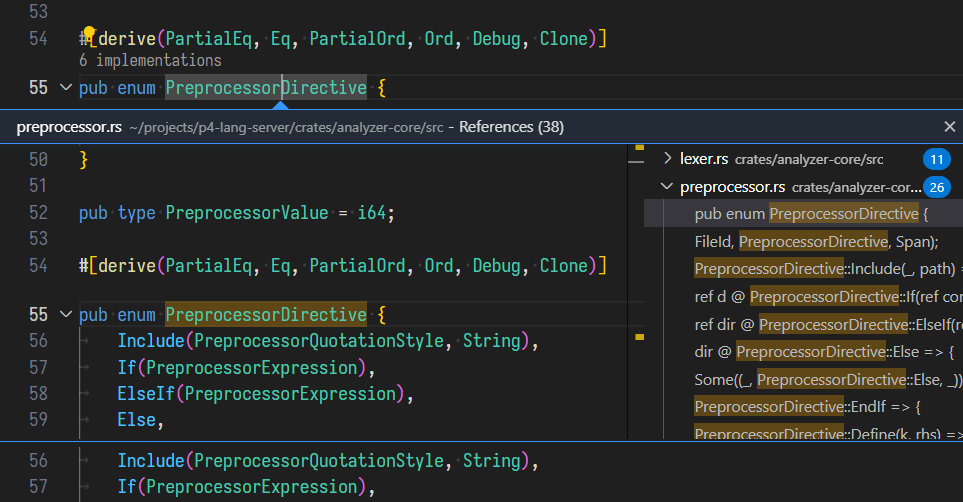
\includegraphics[width=1.00\textwidth]{resources/code_find_references.png}
	\caption{Find References in Visual Studio Code via rust-analyzer.}
\end{figure}

Go to Definition and Find References are
present in some of the oldest code comprehension tools, dating back at least to
the Unix utility \texttt{ctags}\cite{exuberant_ctags}. These let the editor jump
from a symbol's use-site to its definition and vice versa, just as their names
imply. \acrshort{lsp}'s Document Highlight request does not provide syntax
highlighting, rather, it serves to visually assist the programmer with locating
references of a given symbol without having to explicitly invoke the Find
References feature. Document Highlight could be merged with Find References
functionality, but the \acrshort{lsp} maintainers choose to keep them separate
and allow Document Highlight to report imprecise (``fuzzy'') matches. A response
to the Document Link request lists the hyperlinks embedded in the document.
Document Symbols provides a potentially hierarchical overview of the symbols of
a document, which serves the ``outline'' feature of modern editors: a tree
overview of a program's constructs, such as modules, classes, fields, and
methods. The Hover feature provides additional contextual information when
navigating code. It is typically implemented by the client rendering a pop-up
box of documentation for a given symbol. Finally, Code Lens is a versatile
editor feature for displaying additional information at a given position in a
document, such as the number of references of a type or the code metrics of a
procedure\cite{codelens_comparison}. It can trigger an action when activated,
which is used by some servers to run tests or open a Find References dialog.

\begin{figure}[t]\centering
	\begin{multicols}{2}
	\begin{enumerate}
		\item Go to Declaration
		\item Go to Definition \org
		\item Go to Type Definition
		\item Go to Implementation
		\item Find References \org
		\item Prepare Call Hierarchy
		\item Call Hierarchy Incoming Calls
		\item Call Hierarchy Outgoing Calls
		\item Prepare Type Hierarchy
		\item Type Hierarchy Super Types
		\item Type Hierarchy Sub Types
		\item Document Highlight \org
		\item Document Link \org
		\item Document Link Resolve \org
		\item Hover \org
		\item Code Lens \org
		\item Code Lens Refresh
		\item Folding Range
		\item Selection Range
		\item Document Symbols \org
		\item Semantic Tokens
		\item Inlay Hint
		\item Inlay Hint Resolve
		\item Inlay Hint Refresh
		\item Document Color
	\end{enumerate}
	\end{multicols}

	\caption{Code comprehension -related requests in \acrshort{lsp} 3.17.}
	\label{fig:comprehension-requests}
\end{figure}


\subsection{Coding features in \acrshort{lsp}}

A shorter but no less important range of \acrshort{api} calls supports the
developer right when they are authoring code. The main features are
auto-completion, signature help, formatting, and symbol renaming.

\begin{figure}
	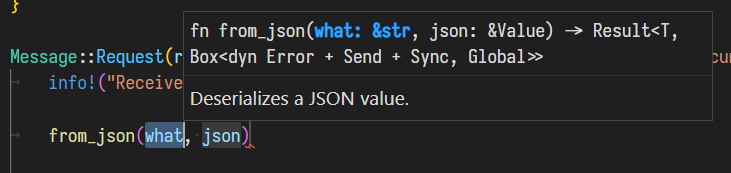
\includegraphics[width=1.00\textwidth]{resources/code_signature_help.png}
	\caption{Signature help in VS Code for Rust shows a pop-up with
	documentation as well as the signature of the callee, highlighting the
	parameter under cursor.}
\end{figure}

Auto-completion offers to fill in code as the programmer is typing, supports
ranking results based on their relevance, on both the server and the client
side, and can include a ``quick info'' description for each option. Signature
help shows parameter name and type information when calling a procedure, method,
or function. Formatting allows a language server to rewrite a document upon
request, for example to conform to a particular code style. The \acrshort{lsp}
formatting functionality can format either the entire document, a selected
range, or reactively an arbitrary part of the document as the user types.
Finally, symbol renaming performs a context-sensitive workspace-wide rename of a
given symbol.

\begin{figure}[t]\centering
	\begin{multicols}{3}
	\begin{enumerate}
		\item Inline Value
		\item Inline Value Refresh
		\item Moniker
		\item Completion Proposals \org
		\item Completion Item Resolve \org
		\item Publish Diagnostics
		\item Pull Diagnostics
		\item Signature Help \org
		\item Code Action
		\item Code Action Resolve
		\item Color Presentation
		\item Formatting \org
		\item Range Formatting \org
		\item On type Formatting \org
		\item Rename \org
		\item Prepare Rename
		\item Linked Editing Range
	\end{enumerate}
	\end{multicols}

	\caption{Coding language features in \acrshort{lsp} 3.17.}
	\label{fig:coding-requests}
\end{figure}

Later \acrshort{lsp} revisions added high-level features not universally
applicable to all programming languages. For instance, version 3.16 added
\emph{linked editing}, which some conforming implementations use to update
opening and closing \acrshort{xml} tags seamlessly without the user specifically
triggering a rename action. Version 3.17 introduced \emph{type hierarchy}
requests, relevant only to programming languages with subtyping. On the other
hand, more general facets of the protocol see creative use in unintended
contexts. One example is the use of lenses and special comments in the Haskell
Language Server project\cite{haskell_ls} to provide \acrshort{repl}-like
functionality. Another is the LT$_\text{E}$X Visual Studio Code
extension\cite{vscode_spellcheck}, which provides spell and grammar checking in
Markdown and \LaTeX{} documents, as well as in programming language comments.
Even though \acrshort{lsp} has no built-in support for extracting the comments
of a document or for spell checking in general, LT$_\text{E}$X achieves this
with a combination of non-\acrshort{lsp} \acrshort{api}s and by leveraging
\acrshort{lsp} diagnostics and code actions to provide suggested spellings.

\begin{figure}[h]\centering
	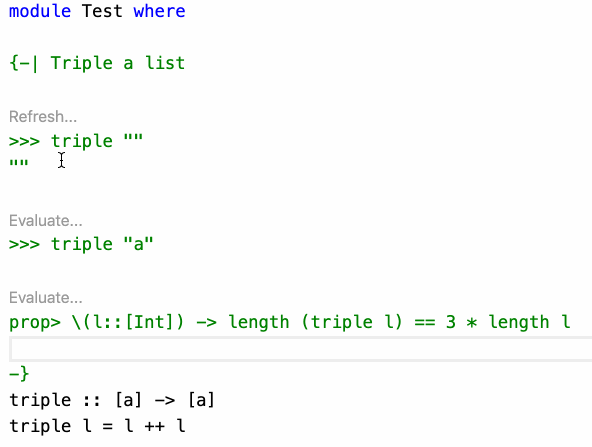
\includegraphics[height=0.3\textheight]{resources/code_haskell_repl.png}
	\caption{The Haskell Language Server project supports in-editor expression
	evaluation in comments prefixed with \texttt{>>>} and checking QuickCheck
	properties in comments starting with \texttt{prop>}.}
\end{figure}

\subsection{The state of the art}

Some of the best tooling in the \acrshort{lsp} ecosystem comes, somewhat
unsurprisingly, from Microsoft.

Projects which served as the de facto \acrshort{ide} integration for the given
language matured somewhat quicker than software that already had ample
competition.

\todo[inline]{the idea here is to compare "actual" language popularity
with the popularity of a corresponding language server.
We should see people preferring other tools for established technologies.}

We have chosen to exclude some technologies from this comparison. JavaScript,
TypeScript, CSS, and HTML support is built into VS Code and therefore does not
show up in VS Code marketplace statistics for installed language extensions.
SQL, while popular, has too many dialects to present a faithful picture through
the lens of extension installations alone. These technologies were in turn
filtered out from StackOverflow's list of most popular languages to highlight
the differences in ranking.

\todo[inline]{
	add the source
	% https://marketplace.visualstudio.com/search?target=VSCode&category=Programming%20Languages&sortBy=Installs
}

\begin{table}\centering
\caption{Popularity of programming languages among VS Code users and
StackOverflow's 2022 Developer survey\cite{stackoverflow_survey_2022}
respondents.}
\begin{tabular}{|r|c|c|}
	Rank & VS Code extension & Most popular programming and scripting languages
	\tabularnewline \hline
	1  & Python     & Python     \tabularnewline
	2  & C/C++      & Java       \tabularnewline
	3  & Java       & C\#        \tabularnewline
	4  & C\#        & C/C++      \tabularnewline
	5  & Go         & PHP        \tabularnewline
	6  & PHP        & PowerShell \tabularnewline
	7  & PowerShell & Go         \tabularnewline
	8  & Dart       & Rust       \tabularnewline
	9  & Ruby       & Dart       \tabularnewline
	10 & Rust       & Ruby       \tabularnewline
\end{tabular}
\end{table}

